\documentclass[11pt, a4paper]{article}
\usepackage[paper=a4paper, left=1.5cm, right=1.5cm, bottom=1.5cm, top=1.5cm]{geometry}

\usepackage[utf8]{inputenc}
\usepackage[T1]{fontenc}
\usepackage[spanish]{babel}
\usepackage[section]{placeins}
\usepackage{caratula/caratula}
\usepackage{listings}
\usepackage{algpseudocode}
\usepackage{graphicx}
\usepackage{float}
\usepackage{amsmath}
%\usepackage{adjustbox}
\usepackage{blindtext}
\usepackage{sidecap}
\usepackage{color}
\usepackage{subfigure}

\usepackage{xspace}
\usepackage{xargs} %Para crear funciones con muchos argumentos
\usepackage{ifthen}
\usepackage{aed2-tad,aed2-symb,aed2-itef,caratula} %Macros de Algo2
\usepackage{algorithm}% http://ctan.org/pkg/algorithms
%\usepackage{algorithmic} %paquete para hacer pseudocodigo
\usepackage{titlesec}%http://foro-c.com/blog/latex-formato-de-titulos-de-capitulos-secciones-etc/
\usepackage{setspace}
\usepackage{fancyhdr}
\usepackage[colorlinks=true, linkcolor=blue]{hyperref} %Links para el indice.
\usepackage{float} %Insercion de imagenes flotantes
\usepackage{ stmaryrd }

\usepackage{caption}
\usepackage{subcaption}

\newcommand{\moduloNombre}[1]{\textbf{#1}}

\let\NombreFuncion=\textsc
\let\TipoVariable=\texttt
\let\ModificadorArgumento=\textbf
\newcommand{\res}{$res$\xspace}
\newcommand{\tab}{\hspace*{7mm}}

\newcommandx{\TipoFuncion}[3]{%
  \NombreFuncion{#1}(#2) \ifx#3\empty\else $\to$ \res\,: \TipoVariable{#3}\fi% nombreFuncion(parametros) -> res:(Tipo)
}
\newcommand{\In}[2]{\ModificadorArgumento{in} \ensuremath{#1}\,: \TipoVariable{#2}\xspace}
\newcommand{\Out}[2]{\ModificadorArgumento{out} \ensuremath{#1}\,: \TipoVariable{#2}\xspace}
\newcommand{\Inout}[2]{\ModificadorArgumento{in/out} \ensuremath{#1}\,: \TipoVariable{#2}\xspace}
\newcommand{\Aplicar}[2]{\NombreFuncion{#1}(#2)}

\newlength{\IntFuncionLengthA}
\newlength{\IntFuncionLengthB}
\newlength{\IntFuncionLengthC}
%InterfazFuncion(nombre, argumentos, valor retorno, precondicion, postcondicion, complejidad, descripcion, aliasing)
\newcommandx{\InterfazFuncion}[9][4=true,6,7,8,9]{%
  \hangindent=\parindent
  \TipoFuncion{#1}{#2}{#3}\\%
  \textbf{Pre} $\equiv$ \{#4\}\\%
  \textbf{Post} $\equiv$ \{#5\}%
  \ifx#6\empty\else\\\textbf{Complejidad:} #6\fi%
  \ifx#7\empty\else\\\textbf{Descripcion:} #7\fi%
  \ifx#8\empty\else\\\textbf{Aliasing:} #8\fi%
  \ifx#9\empty\else\\\textbf{Requiere:} #9\fi%
}

\newenvironment{Algoritmos}{%
  \vspace*{2ex}%
  \noindent\textbf{}%
  \vspace*{2ex}%
}{}

\newcommand{\Titulo}[1]{
  \vspace*{1ex}\par\noindent\textbf{\large #1}\par
}

\newcommand{\DRef}{\ensuremath{\rightarrow}}

\newcommandx{\Algoritmo}[4]{%
	\noindent\TipoFuncion{#1}{#2}{#3}
	\begin{algorithmic}[1]
	#4
	\end{algorithmic}
}%

\newcommand{\nom}[1]{\NombreFuncion{#1}}

\newcommand{\comp}[1]{\hfill \ensuremath{O(#1)}}
\newcommand{\compTot}[1]{\hfill \textbf{Complejidad Total: }\ensuremath{O(#1)}}

\begin{document}

\titulo{Trabajo Práctico \#1}
\fecha{28 de Junio de 2013}
\materia{Sistemas operativos}
% \grupo{Grupo 11}
\integrante{Leandro Matayoshi}{79/11}{leandro.matayoshi@gmail.com}
\integrante{Martin Santos}{413/11}{martin.n.santos@gmail.com}
\integrante{Alexander Szyrej}{642/11}{luzbelito.as@gmail.com}

%Carátula
\maketitle
\newpage
%Indice
\tableofcontents
\newpage


\section{Introducción}
El siguiente trabajo tiene como objetivo realizar una implementación multi-threaded de \textbf{BattleSystem} en base a la single-threaded creada por los $mono-programadores$. Es decir, modificar la implementación existente de manera tal que soporte múltiples threads, para lo cual resulta necesaria la creación de un módulo que permita sincronizar los threads al momento de leer o escribir. 
Así mismo se modificó el servidor para que lance un thread por cada jugador, uno por cada controlador y luego imprima los puntajes totales al finalizar el juego.
Luego se protegio el modelo del juego, haciendo ese módulo $thread-safe$.


\section{RWLock: Lock de lecto-escritura sin inanición}
Se tiene determinada memoria compartida a la cual desean acceder dos tipos de procesos, lectores y escritores. Se deben cumplir las siguientes condiciones:
\begin{itemize}
	\item Solamente puede acceder un escritor al mismo tiempo. Si un lector o un escritor quiere ingresar a la memoria compartida y hay un escritor utilizándola, entonces debe esperar.
	\item Pueden haber varios lectores utilizando la memoria compartida al mismo tiempo, pero si un escritor desea hacer uso de la memoria mientras los lectores la usan, deberá esperar.
\end{itemize}

En otras palabras, la presencia de un $thread$ (lectores) en la memoria compartida no necesariamente excluye el ingreso de otros $threads$ pero, la presencia de determinado tipo de $thread$ (escritores), si lo hace.

Para resolver este problema implementamos dos estructuras de datos (RWLock\_libro y RWLock) que hacen uso de los semáforos POSIX. A continuación presentamos las dos soluciones:

\subsection{Implementación 1} 

En esta implementación utilizamos 3 semáforos y un contador inicializados de la siguiente manera:

\begin{algorithm}[H]
\caption{Inicialización}\label{ej1}
\begin{algorithmic}[1]
\Procedure{Inicialización}{}
	\State turnstile = Semaphore(1)
	\State mutex = Semaphore(1)
	\State roomEmpty = Semaphore(1)
	\State readers = 0
\EndProcedure
\end{algorithmic}
\end{algorithm}

En donde $mutex$ sirve para proteger la variable $readers$, $roomEmpty$ provee acceso exclusivo a la sección crítica y $turnstile$ evita la inanición de los escritores.

\begin{algorithm}[H]
\caption{Writers}\label{ej1}
\begin{algorithmic}[1]
\Procedure{Writers}{}
	\State turnstile.wait()
	\State roomEmpty.wait()
	\State //CRITICAL SECTION
	\State turnstile.signal()
	\State roomEmpty.signal()
\EndProcedure
\end{algorithmic}
\end{algorithm}

Si llega un escritor mientras hay lectores en la sección crítica entonces este se bloquea en la línea 3 esperando el lock de $roomEmpty$. Esto significa que obtuvo el lock de $turnstile$ que impedirá el acceso de más lectores mientras haya un escritor esperando (no hay inanición de escritores). A continuación, el código de los lectores:

\begin{algorithm}[H]
\caption{Readers}\label{ej1}
\begin{algorithmic}[1]
\Procedure{Readers}{}
	\State turnstile.wait()
	\State turnstile.signal()
	\State mutex.wait()
	\State readers++
	\If{readers==1}
		\State roomEmpty.wait()
	\EndIf
	\State mutex.signal()
	\State //CRITICAL SECTION
	\State mutex.wait()
	\State readers$--$
	\If{readers==0}
		\State roomEmpty.signal()
	\EndIf
	\State mutex.signal()
\EndProcedure
\end{algorithmic}
\end{algorithm}

El primer lector en ingresar espera que no haya nadie presente en la sección crítica (línea 6). Cuando el último lector se va, desbloquea $roomEmpty$ permitiendo que ingrese el escritor que estaba esperando. Cuando el escritor se va, desbloquea $turnstile$ permitiendo que cualquiera de los que estaba esperando (sea escritor o lector) acceda a la sección crítica. Esto último nos garantiza que la implementación se encuentra libre de inanición ya que tanto escritores como lectores tendrán acceso garantizado a la memoria compartida y no serán encolados por siempre.

\subsection{Implementación 2}

En esta implementación usamos 4 semáforos ($rw\_lock$, $accessR$, $accessW$ y $mutex$) y 4 contadores ($readers$, $readers\_waiting$, $writers$, $writers\_waiting$).
Incialización:

\begin{algorithm}[H]
\caption{Inicialización}\label{ej1}
\begin{algorithmic}[1]
\Procedure{Inicialización}{}
	\State rw\_lock = Semaphore(1)
	\State accessR = Semaphore(0)
	\State accessW = Semaphore(0)
	\State mutex = Semaphore(1)
	\State readers = 0
	\State readers\_waiting = 0
	\State writers = 0
	\State writers\_waiting = 0
\EndProcedure
\end{algorithmic}
\end{algorithm}

Código para los lectores:

\begin{algorithm}[H]
\caption{Readers}\label{ej1}
\begin{algorithmic}[1]
\Procedure{rlock}{}
	\State mutex.wait()
	\If{writers==0 \&\& writers\_waiting==0}
		\If{readers==0}
			\State rw\_lock.wait()
		\EndIf
		\State readers++
		\State mutex.signal()
	\Else
		\State readers\_waiting++
		\State mutex.signal()
		\State accessR.wait()
		\State mutex.wait()
		\If{readers==0}
			\State rw\_lock.wait()
		\EndIf
		\State readers++
		\State mutex.signal()
	\EndIf
	\State //CRTICAL SECTION
	
\EndProcedure
\end{algorithmic}
\end{algorithm}

Para que un lector pueda acceder a la sección crítica debe cumplirse que no haya escritores esperando ni escribiendo. Si se cumple, entonces se incrementa la variable $readers$ y se accede a la sección crítica. Si no ocurre, se incrementa $readers\_waiting$ y se espera el lock de $accessR$ que será desbloqueado cuando el último escritor salga. Si es el primer lector en llegar, se bloquea aguardando el lock de rw\_lock para cersiorarse de que no haya escritores escribiendo.

\begin{algorithm}[H]
\caption{Readers}\label{ej1}
\begin{algorithmic}[1]
\Procedure{runlock}{}
	\State mutex.wait()
	\State readers $--$
	\If{readers==0}
		\If{writers\_waiting > 0}
			\For{i $\shortleftarrow$ 0 to writers\_waiting}
				\State accessW.signal()
			\EndFor
			\State writers\_waiting $\shortleftarrow$ 0
			\State rw\_lock.signal()
		\EndIf
	\EndIf
	\State mutex.signal()
\EndProcedure
\end{algorithmic}
\end{algorithm}

Cuando el último lector sale verifica si hay escritores esperando. De ser así, tira tantos signals de $accessW$ como escritores haya. Luego reinicia la variable $writers\_waiting$ y desbloquea $rw\_lock$. Escritores:

\begin{algorithm}[H]
\caption{Writers}\label{ej1}
\begin{algorithmic}[1]
\Procedure{wlock}{}
	\State mutex.wait()
	\If{readers==0 \&\& readers\_waiting==0}
		\State writers++
		\State mutex.signal()
		\State rw\_lock.wait()
	\Else
		\State writers\_waiting++
		\State mutex.signal()
		\State accessW.wait()
		\State mutex.wait()
		\State writers++
		\State mutex.signal()
		\State rw\_lock.wait()
	\EndIf
\EndProcedure
\end{algorithmic}
\end{algorithm}

Los escritores realizan un procedimiento similar a los lectores con la diferencia de que solo puede acceder un escritor a la vez. Por lo tanto, siempre deben esperar el lock de $rw\_lock$.

\begin{algorithm}[H]
\caption{Writers}\label{ej1}
\begin{algorithmic}[1]
\Procedure{wunlock}{}
	\State mutex.wait()
	\State writers $--$
	\If{writers==0}
		\If{readers\_waiting > 0}
			\For{i $\shortleftarrow$ 0 to readers\_waiting}
				\State accessR.signal()
			\EndFor
			\State readers\_waiting $\shortleftarrow$ 0
		\EndIf
	\EndIf
	\State rw\_lock.signal()
	\State mutex.signal()
\EndProcedure
\end{algorithmic}
\end{algorithm}

Al igual que los lectores, el último escritor en salir despierta a todos los lectores que estaban esperando y reinicializa la variable $readers\_waiting$. Luego, desbloquea el $rw\_lock$.

\subsection{Tester}

Para corroborar el correcto funcionamiento del RWLock implementamos un tester (testerRW.cpp). Para utilizarlo es necesario pasarle dos parámetros: cantidad de lectores (L) y cantidad de escritores (E). El tester probará lo siguiente:

\begin{itemize}
	\item Que lean los L lectores y luego escriban los E escritores.
	\item Que escriban los E escritores y luego lean los L lectores.
	\item Que lean L/2 lectores y luego que escriban E/2 escritores. Repetir esto paso dos veces.
\end{itemize}

La idea es observar que el algoritmo se encuentre libre de $deadlock$ por lo que al tomar instancias grandes de lectores y escritores el tester no debería tildarse.





\section{Modificando $server.cpp$}
$server.cpp$ es la implementación del ciclo principal del servidor. Su función es establecer las conexiones con los jugadores y controladores y atenderlos mediante dos funciones:

\begin{itemize}
	\item void atender\_jugador(int i): Dado un mensaje del jugador i, ejecuta el comando pedido y envía la respuesta y los eventos pendientes para este jugador.
	\item void void atender\_controlador(): Dado un mensaje del controlador, ejecuta el comando y envía la respuesta.
\end{itemize}

Mediante la creación de varios threads se buscará:

\begin{itemize}
	\item Permitir que múltiples jugadores puedan conectarse al $backend$ de forma simultánea.
	\item Permitir que uno o varios controladores se conecten al backend en cualquier momento sin importar el estado del juego y puedan obtener los puntajes de los jugadores con el comando Get\_Scores.
\end{itemize}

Para ello realizamos diversas modificaciones en el código del server previsto. Disponemos de un $main$ $thread$ encargado de orquestar todo el sistema distribuyendo trabajos a otros $threads$.

Cuando un jugador quiere conectarse al juego el $main$ $thread$ realiza las siguientes operaciones:

\begin{itemize}
	\item[1] Espera que la conexión sea aceptada por el servidor.
	\item[2] Crea un nuevo $thread$ que atiende al jugador entrante mediante la función $atencion\_p$ (Habrá tantos $threads$ como jugadores haya en el sistema).
	\item[3] El jugador es atendido hasta que finalice el juego.
	\item[4] Cuando finaliza el juego, el $thread$ encargado de atender al jugador termina avisándole al $main$ $thread$.
\end{itemize}

Pseudocódigo:

\begin{algorithmic}
  \Function{Jugador}{}
	\State $pthread\_t \ threads[MAX\_JUGADORES]$ 
	\State $int \ tids[MAX\_JUGADORES]$
	\For{jugador = 0 to n}
		\State accept(jugador)
		\State $pthread\_create(\&threads[i],NULL,atencion\_p,\&tids[jugador])$
	\EndFor
  \EndFunction
\end{algorithmic}

La función encargada de atender a los jugadores es:

\begin{algorithmic}
  \Function{atencion\_p}{jugador}
	\State $bool$ $sale$ $=$ $false$ 
	\While {$!sale$}
		\State atender\_jugador(jugador)
		\State sale = model->termino()
	\EndWhile
	\State $pthread\_exit(NULL)$
  \EndFunction
\end{algorithmic}

Habrá un $thread$, creado por el $main$ $thread$, encargado de atender a los controladores de forma similar a la de los jugadores: aceptando la conexión y creando un nuevo $thread$ por cada controlador.

Una vez que todos los $threads$ encargados de atender a los jugadores y controladores finalizan, el $main$ $thread$ termina su ejecución. Para comprender mejor el accionar del server, presentamos un esquema ilustrativo:


\begin{figure}[H]
\centering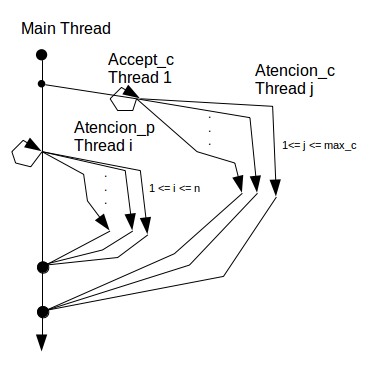
\includegraphics[scale=0.7]{imgs/server.png}
\caption{Esquema del funcionamiento del server.}
\end{figure}


\section{Protegiendo el juego. Un modelo thread-safe.}
Como vimos anteriormente, durante el transcurso del juego se tiene $n + m$ threads que acceden al modelo del juego, donde $n$ es la cantidad de jugadores y $m$ la cantidad de controladores que se conectan. 
Lo que queremos hacer es que el juego no se rompa si varios threads quieren interactuar en simultáneo con los mismos elementos del juego. Por ejemplo queremos evitar inconsistencias en el modelo del juego cuando se conectan dos jugadores y se los agrega al modelo, o cuando dos jugadores ataquen al mismo jugador simultáneamente.

Se utilizaron los siguientes locks para hacer $thread-safe$ el modelo:
\begin{itemize}
	\item	\textbf{lock\_jugadores} es un arreglo de RWLocks, uno por cada jugador, cada uno protege los elementos de cada uno de los jugadores.
	\item	\textbf{lock\_estado\_jugadores} protege la integridad del arreglo de jugadores.
	\item	\textbf{lock\_eventos}, es otro arreglo de RWLocks, asi como el anterior tiene un lock por cada jugador, protege las colas de eventos de cada uno.
	\item	\textbf{lock\_estado\_eventos} protege la integridad del arreglo de eventos.
	\item	\textbf{lock\_jugando} protege la variable jugando (el estado del juego).
\end{itemize}

Dado que nuestra implementación de RWLock no posee un método que transforme un lock de lectura en uno de escritura, si la función que estamos protegiendo hace lecturas de una variable y puede eventualmente modificarla debemos pedir el lock de escritura desde un principio. Esto sucede por ejemplo en las funciones $ubicar$ o $tocar$ donde el juego puede que cambie de estado. En un principio se lee la variable $jugando$ durante el chequeo de errores, verificando que el estado del juego sea el que debe ser. Pero si el último jugador termina de ubicar sus barcos o se produce un toque que elimina al ultimo contrincante el juego cambia de estado. Esto hace que no se permita concurrencia en dichas funciones, y que todas aquellas que hacen chequeos de error al comienzo deban esperar el lock.

\section{Conclusiones}
Implementar un RWLock sin inanici�n es important�simo para el buen desarrollo del juego aqu� presente, m�s aun si se considera que podr�a ser jugado por una cantidad muy grande de jugadores. Varios ataques podr�an no resultar como es esperado si hay ininici�n para los escritores.

Una implementaci�n de un m�todo de transici�n entre estados de lectura y escritura podr�a mejorar la protecci�n y desarrollo del juego, visto y considerando que podr�a por ejemplo permitir m�s concurrencia en la funci�n $ubicar$, donde por el simple hecho de que el �ltimo en ubicar sus barcos inicia el juego y modifica su estado no se permite la lectura en simult�neo de la variable $jugando$ para chequeo de errores. Lo mismo sucede en $tocar$ donde puede que finalice el juego.

Respecto al servidor, nuestra primera implementaci�n resolv�a las conexiones entrantes lanzando primero $n$ threads para cada jugador y el i-�simo thread realizaba el accept del i-�simo jugador. Resolvimos cambiar dicha implementacion para que un �nico thread se quede a la espera de nuevas conexiones y los nuevos threads de atenci�n se lanzan al momento de realizarse el $connect$ de cada uno. De esta manera no se tiene desde el principio $n$ threads $inactivos$ bloqueados. Algo similar sucede con los controladores, m�s importante es aun dado que no tenemos la certeza de cuantos controladores se conectar�n al juego.

\end{document}
